\documentclass{extbook}[14pt]
\usepackage{multicol, enumerate, enumitem, hyperref, color, soul, setspace, parskip, fancyhdr, amssymb, amsthm, amsmath, latexsym, units, mathtools}
\everymath{\displaystyle}
\usepackage[headsep=0.5cm,headheight=0cm, left=1 in,right= 1 in,top= 1 in,bottom= 1 in]{geometry}
\usepackage{dashrule}  % Package to use the command below to create lines between items
\newcommand{\litem}[1]{\item #1

\rule{\textwidth}{0.4pt}}
\pagestyle{fancy}
\lhead{}
\chead{Answer Key for Progress Quiz 5 Version B}
\rhead{}
\lfoot{8497-6012}
\cfoot{}
\rfoot{Summer C 2021}
\begin{document}
\textbf{This key should allow you to understand why you choose the option you did (beyond just getting a question right or wrong). \href{https://xronos.clas.ufl.edu/mac1105spring2020/courseDescriptionAndMisc/Exams/LearningFromResults}{More instructions on how to use this key can be found here}.}

\textbf{If you have a suggestion to make the keys better, \href{https://forms.gle/CZkbZmPbC9XALEE88}{please fill out the short survey here}.}

\textit{Note: This key is auto-generated and may contain issues and/or errors. The keys are reviewed after each exam to ensure grading is done accurately. If there are issues (like duplicate options), they are noted in the offline gradebook. The keys are a work-in-progress to give students as many resources to improve as possible.}

\rule{\textwidth}{0.4pt}

\begin{enumerate}\litem{
Solve the rational equation below. Then, choose the interval(s) that the solution(s) belongs to.
\[ \frac{-20}{70x -40} + 1 = \frac{-20}{70x -40} \]The solution is \( \text{all solutions are invalid or lead to complex values in the equation.} \), which is option A.\begin{enumerate}[label=\Alph*.]
\item \( \text{All solutions lead to invalid or complex values in the equation.} \)

*$x = 0.571$ leads to dividing by 0 in the original equation and thus is not a valid solution, which is the correct option.
\item \( x \in [0.57,1.57] \)

$x = 0.571$, which corresponds to not checking if this value leads to dividing by 0 in the original equation and thus is not a valid solution.
\item \( x_1 \in [0.4, 1.1] \text{ and } x_2 \in [0.57,1.57] \)

$x = 0.571 \text{ and } x = 0.571$, which corresponds to getting the correct solution and believing there should be a second solution to the equation.
\item \( x \in [-1.6,0.3] \)

$x = -0.571$, which corresponds to not distributing the factor $70x -40$ correctly when trying to eliminate the fraction.
\item \( x_1 \in [-1.6, 0.3] \text{ and } x_2 \in [0.57,1.57] \)

$x = -0.571 \text{ and } x = 0.571$, which corresponds to getting the correct solution and believing there should be a second solution to the equation.
\end{enumerate}

\textbf{General Comment:} Distractors are different based on the number of solutions. Remember that after solving, we need to make sure our solution does not make the original equation divide by zero!
}
\litem{
Choose the equation of the function graphed below.

\begin{center}
    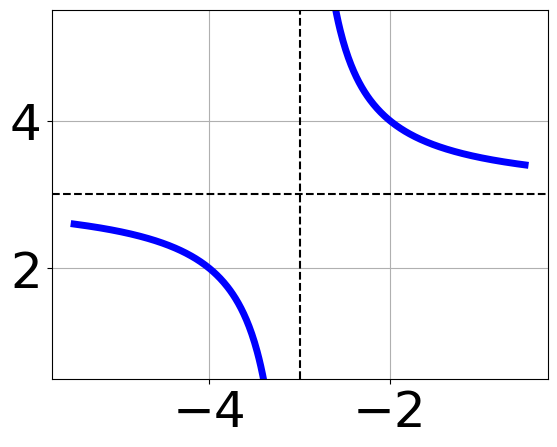
\includegraphics[width=0.5\textwidth]{../Figures/rationalGraphToEquationB.png}
\end{center}


The solution is \( f(x) = \frac{1}{x + 3} + 3 \), which is option C.\begin{enumerate}[label=\Alph*.]
\item \( f(x) = \frac{1}{(x + 3)^2} + 3 \)

Corresponds to thinking the graph was a shifted version of $\frac{1}{x^2}$.
\item \( f(x) = \frac{-1}{x - 3} + 3 \)

Corresponds to using the general form $f(x) = \frac{a}{x+h}+k$ and the opposite leading coefficient.
\item \( f(x) = \frac{1}{x + 3} + 3 \)

This is the correct option.
\item \( f(x) = \frac{-1}{(x - 3)^2} + 3 \)

Corresponds to thinking the graph was a shifted version of $\frac{1}{x^2}$, using the general form $f(x) = \frac{a}{x+h}+k$, and the opposite leading coefficient.
\item \( \text{None of the above} \)

This corresponds to believing the vertex of the graph was not correct.
\end{enumerate}

\textbf{General Comment:} Remember that the general form of a basic rational equation is $ f(x) = \frac{a}{(x-h)^n} + k$, where $a$ is the leading coefficient (and in this case, we assume is either $1$ or $-1$), $n$ is the degree (in this case, either $1$ or $2$), and $(h, k)$ is the intersection of the asymptotes.
}
\litem{
Choose the equation of the function graphed below.

\begin{center}
    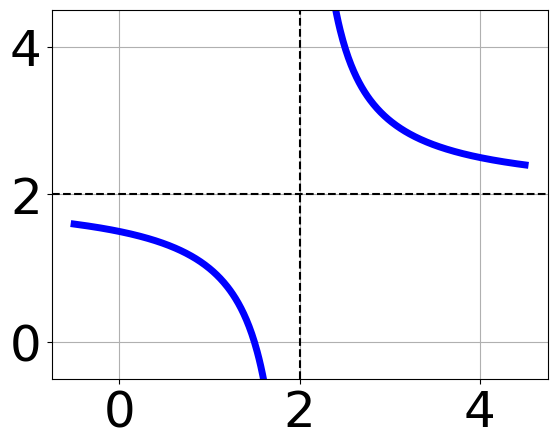
\includegraphics[width=0.5\textwidth]{../Figures/rationalGraphToEquationCopyB.png}
\end{center}


The solution is \( \text{None of the above as it should be } f(x) = \frac{1}{x - 2} + 2 \), which is option E.\begin{enumerate}[label=\Alph*.]
\item \( f(x) = \frac{-1}{(x - 2)^2} + 2 \)

Corresponds to thinking the graph was a shifted version of $\frac{1}{x^2}$, using the general form $f(x) = \frac{a}{x-h}+k$, and the opposite leading coefficient.
\item \( f(x) = \frac{1}{x + 2} + 2 \)

The $x$-value of the equation does not match the graph.
\item \( f(x) = \frac{-1}{x - 2} + 2 \)

Corresponds to using the general form $f(x) = \frac{a}{x-h}+k$ and the opposite leading coefficient.
\item \( f(x) = \frac{1}{(x + 2)^2} + 2 \)

Corresponds to thinking the graph was a shifted version of $\frac{1}{x^2}$.
\item \( \text{None of the above} \)

None of the equation options were the correct equation.
\end{enumerate}

\textbf{General Comment:} Remember that the general form of a basic rational equation is $ f(x) = \frac{a}{(x-h)^n} + k$, where $a$ is the leading coefficient (and in this case, we assume is either $1$ or $-1$), $n$ is the degree (in this case, either $1$ or $2$), and $(h, k)$ is the intersection of the asymptotes.
}
\litem{
Choose the graph of the equation below.
\[ f(x) = \frac{-1}{(x + 3)^2} + 1 \]The solution is the graph below, which is option B.
    \begin{center}
        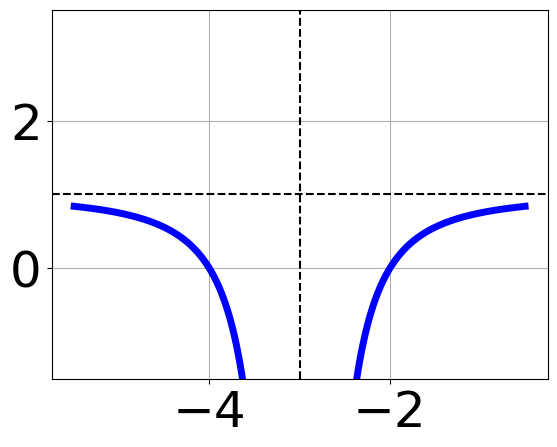
\includegraphics[width=0.3\textwidth]{../Figures/rationalEquationToGraphCopyBB.png}
    \end{center}\begin{enumerate}[label=\Alph*.]
\begin{multicols}{2}
\item 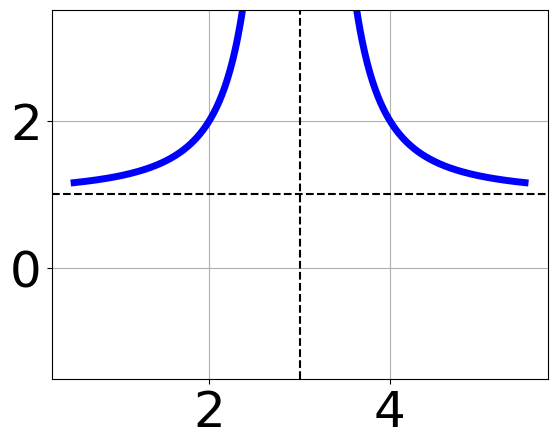
\includegraphics[width = 0.3\textwidth]{../Figures/rationalEquationToGraphCopyAB.png}
\item 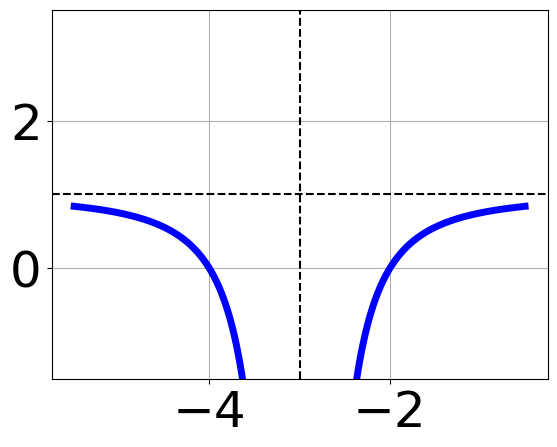
\includegraphics[width = 0.3\textwidth]{../Figures/rationalEquationToGraphCopyBB.png}
\item 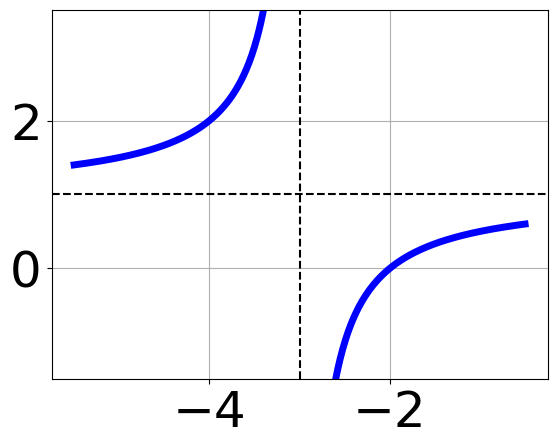
\includegraphics[width = 0.3\textwidth]{../Figures/rationalEquationToGraphCopyCB.png}
\item 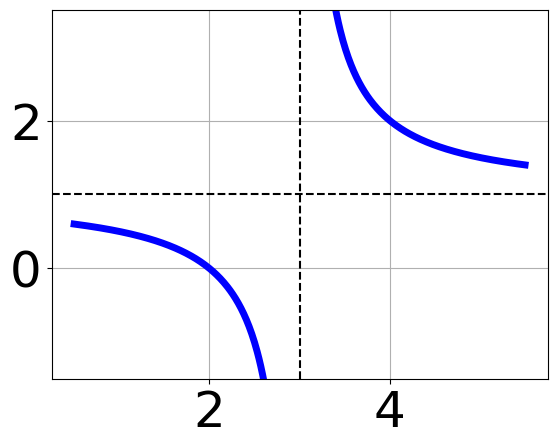
\includegraphics[width = 0.3\textwidth]{../Figures/rationalEquationToGraphCopyDB.png}
\end{multicols}\item None of the above.\end{enumerate}
\textbf{General Comment:} Remember that the general form of a basic rational equation is $ f(x) = \frac{a}{(x-h)^n} + k$, where $a$ is the leading coefficient (and in this case, we assume is either $1$ or $-1$), $n$ is the degree (in this case, either $1$ or $2$), and $(h, k)$ is the intersection of the asymptotes.
}
\litem{
Solve the rational equation below. Then, choose the interval(s) that the solution(s) belongs to.
\[ \frac{-4x}{-5x -5} + \frac{-6x^{2}}{-30x^{2} -60 x -30} = \frac{-2}{6x + 6} \]The solution is \( \text{All solutions are invalid or lead to complex values in the equation.} \), which is option A.\begin{enumerate}[label=\Alph*.]
\item \( \text{All solutions lead to invalid or complex values in the equation.} \)

* The equation leads to solving $-18x^{2} -34 x -10=0$, which leads to complex solutions. This is the correct option.
\item \( x \in [-1.37,-0.95] \)

$x = -1.000$, which corresponds to solving $-5x -5 = 0$ and treating it as a solution to the equation.
\item \( x_1 \in [-0.62, -0] \text{ and } x_2 \in [-1.92,-1.48] \)

$x = -0.364 \text{ and } x = -1.524$, which corresponds to making the discriminant from the Quadratic Formula positive to avoid complex solutions.
\item \( x_1 \in [-1.37, -0.95] \text{ and } x_2 \in [-1.41,-0.89] \)

$x = -1.000 \text{ and } x = -1.000$, which corresponds to solving $-5x -5 = 0$ and $6x + 6 = 0$ and treating them as solutions to the equation.
\item \( x \in [-1.37,-0.95] \)

$x = -1.000$, which corresponds to solving $6x + 6 = 0$ and treating it as a solution to the equation.
\end{enumerate}

\textbf{General Comment:} Distractors are different based on the number of solutions. Remember that after solving, we need to make sure our solution does not make the original equation divide by zero!
}
\litem{
Solve the rational equation below. Then, choose the interval(s) that the solution(s) belongs to.
\[ \frac{-5x}{-3x -5} + \frac{-4x^{2}}{-9x^{2} -27 x -20} = \frac{-4}{3x + 4} \]The solution is \( \text{All solutions are invalid or lead to complex values in the equation.} \), which is option B.\begin{enumerate}[label=\Alph*.]
\item \( x_1 \in [-2.51, -1.62] \text{ and } x_2 \in [-1.47,-1.31] \)

$x = -1.667 \text{ and } x = -1.333$, which corresponds to solving $-3x -5 = 0$ and $3x + 4 = 0$ and treating them as solutions to the equation.
\item \( \text{All solutions lead to invalid or complex values in the equation.} \)

* The equation leads to solving $-11x^{2} -32 x -20=0$, which leads to complex solutions. This is the correct option.
\item \( x_1 \in [-1.11, -0.28] \text{ and } x_2 \in [-2.5,-1.79] \)

$x = -0.909 \text{ and } x = -2.000$, which corresponds to making the discriminant from the Quadratic Formula positive to avoid complex solutions.
\item \( x \in [-1.37,-1.16] \)

$x = -1.333$, which corresponds to solving $3x + 4 = 0$ and treating it as a solution to the equation.
\item \( x \in [-2.51,-1.62] \)

$x = -1.667$, which corresponds to solving $-3x -5 = 0$ and treating it as a solution to the equation.
\end{enumerate}

\textbf{General Comment:} Distractors are different based on the number of solutions. Remember that after solving, we need to make sure our solution does not make the original equation divide by zero!
}
\litem{
Determine the domain of the function below.
\[ f(x) = \frac{4}{24x^{2} +30 x + 9} \]The solution is \( \text{All Real numbers except } x = -0.750 \text{ and } x = -0.500. \), which is option B.\begin{enumerate}[label=\Alph*.]
\item \( \text{All Real numbers except } x = a \text{ and } x = b, \text{ where } a \in [-18.59, -17.66] \text{ and } b \in [-12.34, -11.94] \)

All Real numbers except $x = -18.000$ and $x = -12.000$, which corresponds to not factoring the denominator correctly.
\item \( \text{All Real numbers except } x = a \text{ and } x = b, \text{ where } a \in [-1.29, -0.59] \text{ and } b \in [-0.73, 0.43] \)

All Real numbers except $x = -0.750$ and $x = -0.500$, which is the correct option.
\item \( \text{All Real numbers except } x = a, \text{ where } a \in [-18.59, -17.66] \)

All Real numbers except $x = -18.000$, which corresponds to removing a distractor value from the denominator.
\item \( \text{All Real numbers except } x = a, \text{ where } a \in [-1.29, -0.59] \)

All Real numbers except $x = -0.750$, which corresponds to removing only 1 value from the denominator.
\item \( \text{All Real numbers.} \)

This corresponds to thinking the denominator has complex roots or that rational functions have a domain of all Real numbers.
\end{enumerate}

\textbf{General Comment:} Recall that dividing by zero is not a real number. Therefore the domain is all real numbers \textbf{except} those that make the denominator 0.
}
\litem{
Determine the domain of the function below.
\[ f(x) = \frac{6}{15x^{2} -35 x + 20} \]The solution is \( \text{All Real numbers except } x = 1.000 \text{ and } x = 1.333. \), which is option B.\begin{enumerate}[label=\Alph*.]
\item \( \text{All Real numbers except } x = a \text{ and } x = b, \text{ where } a \in [11.97, 12.02] \text{ and } b \in [24.92, 26] \)

All Real numbers except $x = 12.000$ and $x = 25.000$, which corresponds to not factoring the denominator correctly.
\item \( \text{All Real numbers except } x = a \text{ and } x = b, \text{ where } a \in [0.06, 1.24] \text{ and } b \in [1.27, 1.5] \)

All Real numbers except $x = 1.000$ and $x = 1.333$, which is the correct option.
\item \( \text{All Real numbers except } x = a, \text{ where } a \in [0.06, 1.24] \)

All Real numbers except $x = 1.000$, which corresponds to removing only 1 value from the denominator.
\item \( \text{All Real numbers except } x = a, \text{ where } a \in [11.97, 12.02] \)

All Real numbers except $x = 12.000$, which corresponds to removing a distractor value from the denominator.
\item \( \text{All Real numbers.} \)

This corresponds to thinking the denominator has complex roots or that rational functions have a domain of all Real numbers.
\end{enumerate}

\textbf{General Comment:} Recall that dividing by zero is not a real number. Therefore the domain is all real numbers \textbf{except} those that make the denominator 0.
}
\litem{
Choose the graph of the equation below.
\[ f(x) = \frac{-1}{x - 2} - 1 \]The solution is the graph below, which is option E.
    \begin{center}
        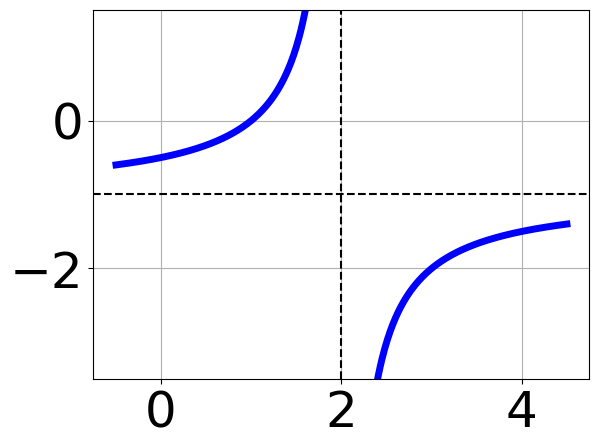
\includegraphics[width=0.3\textwidth]{../Figures/rationalEquationToGraphEB.png}
    \end{center}\begin{enumerate}[label=\Alph*.]
\begin{multicols}{2}
\item 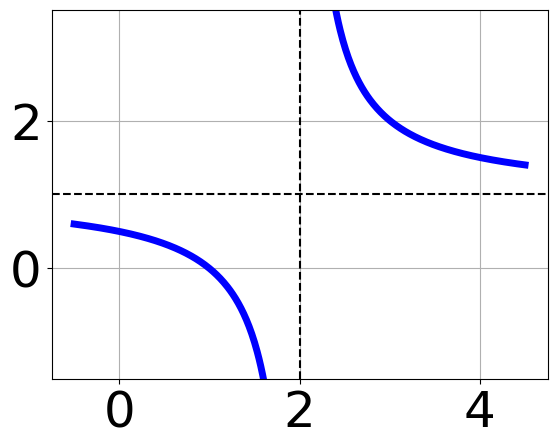
\includegraphics[width = 0.3\textwidth]{../Figures/rationalEquationToGraphAB.png}
\item 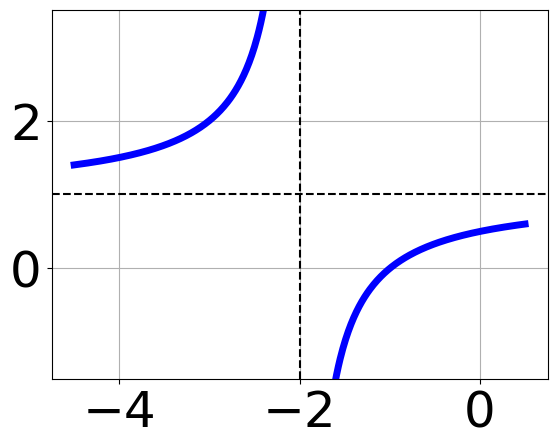
\includegraphics[width = 0.3\textwidth]{../Figures/rationalEquationToGraphBB.png}
\item 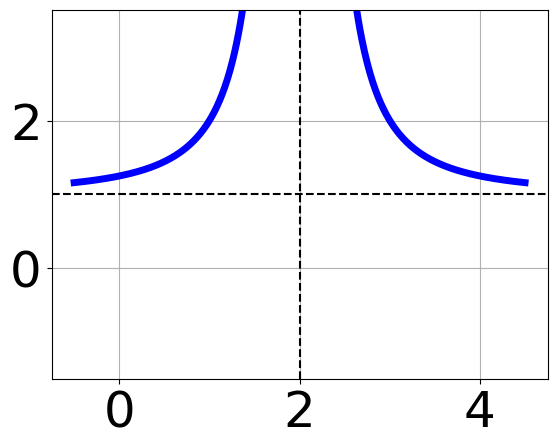
\includegraphics[width = 0.3\textwidth]{../Figures/rationalEquationToGraphCB.png}
\item 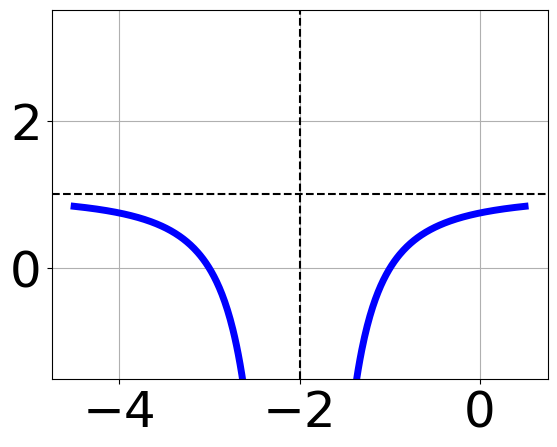
\includegraphics[width = 0.3\textwidth]{../Figures/rationalEquationToGraphDB.png}
\end{multicols}\item None of the above.\end{enumerate}
\textbf{General Comment:} Remember that the general form of a basic rational equation is $ f(x) = \frac{a}{(x-h)^n} + k$, where $a$ is the leading coefficient (and in this case, we assume is either $1$ or $-1$), $n$ is the degree (in this case, either $1$ or $2$), and $(h, k)$ is the intersection of the asymptotes.
}
\litem{
Solve the rational equation below. Then, choose the interval(s) that the solution(s) belongs to.
\[ \frac{-7}{-9x -4} + -6 = \frac{-3}{-36x -16} \]The solution is \( x = -0.329 \), which is option D.\begin{enumerate}[label=\Alph*.]
\item \( x_1 \in [-0.37, -0.32] \text{ and } x_2 \in [-0.3,1.2] \)

$x = -0.329 \text{ and } x = 0.560$, which corresponds to getting the correct solution and believing there should be a second solution to the equation.
\item \( x \in [0.51,0.59] \)

$x = 0.560$, which corresponds to not distributing the factor $-9x -4$ correctly when trying to eliminate the fraction.
\item \( \text{All solutions lead to invalid or complex values in the equation.} \)

This corresponds to thinking $x = -0.329$ leads to dividing by zero in the original equation, which it does not.
\item \( x \in [-0.33,1.67] \)

* $x = -0.329$, which is the correct option.
\item \( x_1 \in [-0.42, -0.36] \text{ and } x_2 \in [-1.1,0.3] \)

$x = -0.370 \text{ and } x = -0.329$, which corresponds to getting the correct solution and believing there should be a second solution to the equation.
\end{enumerate}

\textbf{General Comment:} Distractors are different based on the number of solutions. Remember that after solving, we need to make sure our solution does not make the original equation divide by zero!
}
\end{enumerate}

\end{document}